

\tikzset{every picture/.style={line width=0.75pt}} %set default line width to 0.75pt        
\begin{center}
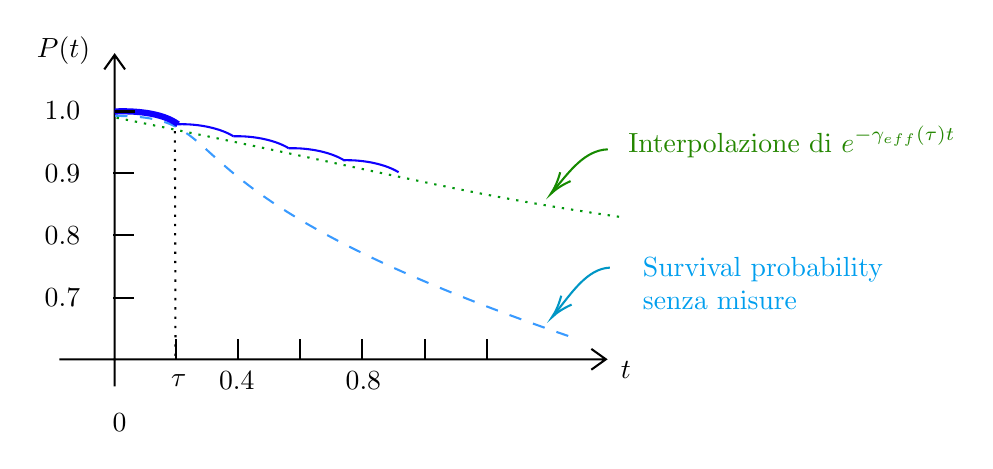
\begin{tikzpicture}[x=0.75pt,y=0.75pt,yscale=-1,xscale=1]
%uncomment if require: \path (0,300); %set diagram left start at 0, and has height of 300

%Shape: Axis 2D [id:dp21522982327423357] 
\draw  (121,175.67) -- (384.33,175.67)(147.67,29) -- (147.67,188.67) (377.33,170.67) -- (384.33,175.67) -- (377.33,180.67) (142.67,36) -- (147.67,29) -- (152.67,36)  ;
%Curve Lines [id:da15785243874113397] 
\draw [color={rgb, 255:red, 57; green, 154; blue, 255 }  ,draw opacity=1 ] [dash pattern={on 4.5pt off 4.5pt}]  (147.84,58.4) .. controls (211.43,58.4) and (159.31,93.88) .. (370.38,165.86) ;


%Curve Lines [id:da8350402313780105] 
\draw [color={rgb, 255:red, 15; green, 0; blue, 255 }  ,draw opacity=1 ][line width=2.25]    (147.68,56.27) .. controls (156.47,55.9) and (170.29,56.57) .. (178.23,62.42) ;


%Curve Lines [id:da6358485219303893] 
\draw [color={rgb, 255:red, 15; green, 0; blue, 255 }  ,draw opacity=1 ]   (178.23,62.42) .. controls (188.78,62.12) and (199,64.56) .. (204.88,68.21) ;


%Curve Lines [id:da4404463330552182] 
\draw [color={rgb, 255:red, 15; green, 0; blue, 255 }  ,draw opacity=1 ]   (204.88,68.21) .. controls (215.43,67.91) and (225.64,70.34) .. (231.53,73.99) ;


%Curve Lines [id:da9745888558673619] 
\draw [color={rgb, 255:red, 15; green, 0; blue, 255 }  ,draw opacity=1 ]   (231.53,73.99) .. controls (242.07,73.69) and (252.29,76.12) .. (258.17,79.77) ;


%Curve Lines [id:da3527462322133508] 
\draw [color={rgb, 255:red, 15; green, 0; blue, 255 }  ,draw opacity=1 ]   (257.81,79.76) .. controls (268.36,79.46) and (278.58,81.89) .. (284.46,85.54) ;


%Straight Lines [id:da34568675396501636] 
\draw  [dash pattern={on 0.84pt off 2.51pt}]  (176.69,65.72) -- (177,176) ;


%Curve Lines [id:da052117335217273464] 
\draw [color={rgb, 255:red, 0; green, 150; blue, 12 }  ,draw opacity=1 ][line width=0.75]  [dash pattern={on 0.84pt off 2.51pt}]  (148.61,59.31) .. controls (287.18,87.19) and (313.34,95.81) .. (391.17,107.06) ;


%Straight Lines [id:da6118859076103123] 
\draw    (147,146) -- (157,146) ;


%Straight Lines [id:da17183505389897635] 
\draw    (147,116) -- (157,116) ;


%Straight Lines [id:da4284019112663999] 
\draw    (147,86) -- (157,86) ;


%Straight Lines [id:da2724371012042419] 
\draw    (147.68,56.27) -- (157.68,56.27) ;


%Straight Lines [id:da45937983782048275] 
\draw    (237,176) -- (237,166) ;


%Straight Lines [id:da9979635498053909] 
\draw    (207,176) -- (207,166) ;


%Straight Lines [id:da7060313167766665] 
\draw    (177,176) -- (177,166) ;


%Straight Lines [id:da27852080941520097] 
\draw    (267,176) -- (267,166) ;


%Straight Lines [id:da4124681634033196] 
\draw    (297,176) -- (297,166) ;


%Straight Lines [id:da7767131492541457] 
\draw    (327,176) -- (327,166) ;


%Curve Lines [id:da4361033074713996] 
\draw [color={rgb, 255:red, 22; green, 138; blue, 0 }  ,draw opacity=1 ]   (385.25,74.5) .. controls (374.09,74.97) and (366.99,84.93) .. (359.02,94.49) ;
\draw [shift={(357.75,96)}, rotate = 310.36] [color={rgb, 255:red, 22; green, 138; blue, 0 }  ,draw opacity=1 ][line width=0.75]    (10.93,-3.29) .. controls (6.95,-1.4) and (3.31,-0.3) .. (0,0) .. controls (3.31,0.3) and (6.95,1.4) .. (10.93,3.29)   ;

%Curve Lines [id:da44210673825584834] 
\draw [color={rgb, 255:red, 0; green, 150; blue, 197 }  ,draw opacity=1 ]   (386.25,131.5) .. controls (375.09,131.98) and (367.54,144.18) .. (359.52,153.98) ;
\draw [shift={(358.25,155.5)}, rotate = 310.36] [color={rgb, 255:red, 0; green, 150; blue, 197 }  ,draw opacity=1 ][line width=0.75]    (10.93,-3.29) .. controls (6.95,-1.4) and (3.31,-0.3) .. (0,0) .. controls (3.31,0.3) and (6.95,1.4) .. (10.93,3.29)   ;


% Text Node
\draw (122.5,56) node   {$1.0$};
% Text Node
\draw (122.5,86) node   {$0.9$};
% Text Node
\draw (122.5,116) node   {$0.8$};
% Text Node
\draw (122.5,146) node   {$0.7$};
% Text Node
\draw (150,206) node   {$0$};
% Text Node
\draw (178.5,186) node   {$\tau $};
% Text Node
\draw (206.5,186) node   {$0.4$};
% Text Node
\draw (267.5,186) node   {$0.8$};
% Text Node
\draw (460,139) node [color={rgb, 255:red, 0; green, 158; blue, 238 }  ,opacity=1 ] [align=left] {Survival probability\\senza misure};
% Text Node
\draw (474,71) node [color={rgb, 255:red, 36; green, 134; blue, 0 }  ,opacity=1 ] [align=left] {Interpolazione di $\displaystyle e^{-\gamma _{\text{eff}}( \tau ) t}$};
% Text Node
\draw (394,181) node   {$t$};
% Text Node
\draw (123,27) node   {$P( t)$};


\end{tikzpicture}
\end{center}